\documentclass[16pt]{beamer}
\usepackage[utf8]{inputenc}

\title{Aspirateurs et pompes à vide}

\usetheme{default}

\usepackage[utf8]{inputenc}
\usepackage{amsmath}
\usepackage{amsfonts}
\usepackage{amssymb}
\usepackage{pgf}
\usepackage{color}
\usepackage[frenchb]{babel}
\usepackage{amssymb}
\usepackage{hyperref}

\usefonttheme{default}
\usepackage{DejaVuSans}
%\usepackage[sfdefault]{FiraSans} %% option 'sfdefault' activates Fira Sans as the default text font
\usepackage[T1]{fontenc}
\renewcommand*\oldstylenums[1]{{\firaoldstyle #1}}


\setbeamertemplate{navigation symbols}{} %remove navigation symbols

\author{Cédric Jeanneret (aka \href{https://www.twitter.com/SwissTengu}{@SwissTengu})}
\institute{\href{https://www.ethack.org/}{EthACK.org}}
\date{\today}

\definecolor{linecolor}{HTML}{4d4c4c}

\setbeamercolor{linecolor}{fg=white,bg=linecolor}

\setbeamertemplate{headline} {
	\begin{beamercolorbox}[wd=\paperwidth,dp=8pt,ht=12pt,leftskip=.29cm,rightskip=.29cm]{linecolor}
	\hfill
	\hypersetup{
		colorlinks=true,
		linkcolor=white,
		urlcolor=white,
	}
	\insertinstitute
	\end{beamercolorbox}%
}

\setbeamertemplate{footline}{%
	\begin{beamercolorbox}[wd=\paperwidth,dp=9pt,ht=0.4cm,leftskip=.29cm,rightskip=.3cm]{linecolor}
	\pgfputat{\pgfxy(0.455,-0.315)}{\pgfbox[center,base]{
\includegraphics[width=1.5cm]{../common/logo_537.png}}}
	\hfill
	\inserttitle
	\end{beamercolorbox}%
}


\hypersetup{
	colorlinks=true,
	linkcolor=blue,
	urlcolor=blue,
	pdfborderstyle={/S/U/W 1},
	pdfborder=0 0 1,
	linkbordercolor={0 0 0},
	urlbordercolor={0 0 0},
}


\begin{document}

{
\setbeamertemplate{footline}{%
	\begin{beamercolorbox}[wd=\paperwidth,dp=8pt,ht=12pt,leftskip=.29cm,rightskip=.3cm]{linecolor}
	\hfill
	\inserttitle
	\end{beamercolorbox}%
}

% center first slide — not a title, but almost
{
\centering
\begin{frame}

EthACK
\vspace{0.5cm}

The Swiss Privacy Basecamp 
\vspace{0.5cm}


\includegraphics[width=4cm]{../common/logo_537.png}

\end{frame}
}
}

\begin{frame}{EthACK ?}
\begin{itemize}
	\item Éthique
	\item État
	\item ACKnowledgement (reconnaissance)
	\item Hacking (éthique, évidemment)
	\item …
\end{itemize}
\end{frame}

\begin{frame}{Pourquoi ?}
\begin{itemize}
	\item Notre gouvernement ne s'intéresse pas (ou peu) au sujet
	\item Les sociétés privées nous fichent à notre insu
	\item Personne ne sait où sont leurs données, qui les traitent, à quoi elles servent
\end{itemize}
\end{frame}


\begin{frame}
  \titlepage
\end{frame}

\begin{frame}
{Plan rapide}
\begin{itemize}
\item Vos données
\note[item]{Ce que vous renseignez, ce qu'on apprend de vous}
\item Usages évidents
\note[item]{Les usages évidents par le réseau et ses membres}
\item Usages moins évidents
\note[item]{Les usages dangereux}
\item Exemples
\note[item]{Quelques exemples tirés de la vie courante}
\item Questions
\end{itemize}
\end{frame}

\begin{frame}
{Vos données et le réseau}
\begin{itemize}
\item Données personnelles "Publiques"
\note[item]{Nom, prénom, adresse, etc}
\item Données personnelles "Privées"
\note[item]{Photos, emploi du temps, etc}
\end{itemize}
\end{frame}

\begin{frame}
{Données déduites}
\begin{itemize}
\item Votre emploi du temps
\note[item]{Où, quand, quoi, comment, avec qui}
\item Votre emplacement
\note[item]{Si vous ne la transmettez pas déjà}
\item Vos futures sorties, vacances, etc
\note[item]{Si vous commencez à parler de tel lieu, telle période, etc}
\end{itemize}
\end{frame}

\begin{frame}
{Utilité de ces données}
\begin{itemize}
\item Découverte de contacts
\note[item]{Recherche possible via nom, prénom, import d'adresses mails, activités, etc, etc}
\item Publicité
\note[item]{Vos centres d'intérêt, promotion, etc}
\item Garder le contact
\note[item]{Une fois le réseau monté, il faut le maintenir}
\end{itemize}
\end{frame}

\begin{frame}
{Usages moins connus}
\begin{itemize}
\item Employeur
\note[item]{RH recherchent infos}
\item Conjoint
\note[item]{Idem}
\item Voleurs
\note[item]{Quoi de mieux que de savoir quand vous êtes chez vous}
\item Scam, Spam, Phishing, etc
\note[item]{Sans doute le + dangereux}
\end{itemize}
\end{frame}

\begin{frame}
{Votre futur employeur}
\begin{itemize}
\item Recherche sur G***e ou autres
\item Tombe sur votre profile
\end{itemize}
\end{frame}

{
\hypersetup{
        colorlinks=true,
        linkcolor=white,
        urlcolor=white
}
\setbeamertemplate{headline} {
        \begin{beamercolorbox}[wd=\paperwidth,dp=8pt,ht=12pt,leftskip=.29cm,rightskip=.29cm]{linecolor}
        \#facebookDrunk :)
        \hfill
        \insertinstitute
        \end{beamercolorbox}%
}
\begin{frame}
\centering

\includegraphics[width=\textwidth,height=\textheight,keepaspectratio]{./facebook-drunk.jpg} 
\end{frame}
}

{
\hypersetup{
        colorlinks=true,
        linkcolor=white,
        urlcolor=white
}
\setbeamertemplate{headline} {
        \begin{beamercolorbox}[wd=\paperwidth,dp=8pt,ht=12pt,leftskip=.29cm,rightskip=.29cm]{linecolor}
        MOAARRR :)
        \hfill
        \insertinstitute
        \end{beamercolorbox}%
}
\begin{frame}
\centering

\includegraphics[width=\textwidth,height=\textheight,keepaspectratio]{./post-drunk.jpg} 
\end{frame}
}
{
\hypersetup{
        colorlinks=true,
        linkcolor=white,
        urlcolor=white
}
\setbeamertemplate{headline} {
        \begin{beamercolorbox}[wd=\paperwidth,dp=8pt,ht=12pt,leftskip=.29cm,rightskip=.29cm]{linecolor}
        Moralité
        \hfill
        \insertinstitute
        \end{beamercolorbox}%
}

\begin{frame}
\centering

\includegraphics[width=\textwidth,height=\textheight,keepaspectratio]{./funny-drunk-Facebook-status.jpg} 
\end{frame}
}

\begin{frame}
{Mais pas seulement vous !}
\begin{itemize}
\item Vos amis et proches
\note[item]{Les tags sur les photos}
\item Soyez informés !
\note[item]{Confirmation tag photo (privacy settings)}
\end{itemize}
\end{frame}

{
\hypersetup{
        colorlinks=true,
        linkcolor=white,
        urlcolor=white
}
\setbeamertemplate{headline} {
        \begin{beamercolorbox}[wd=\paperwidth,dp=8pt,ht=12pt,leftskip=.29cm,rightskip=.29cm]{linecolor}
        Exemple de configuration
        \hfill
        \insertinstitute
        \end{beamercolorbox}%
}

\begin{frame}
\centering
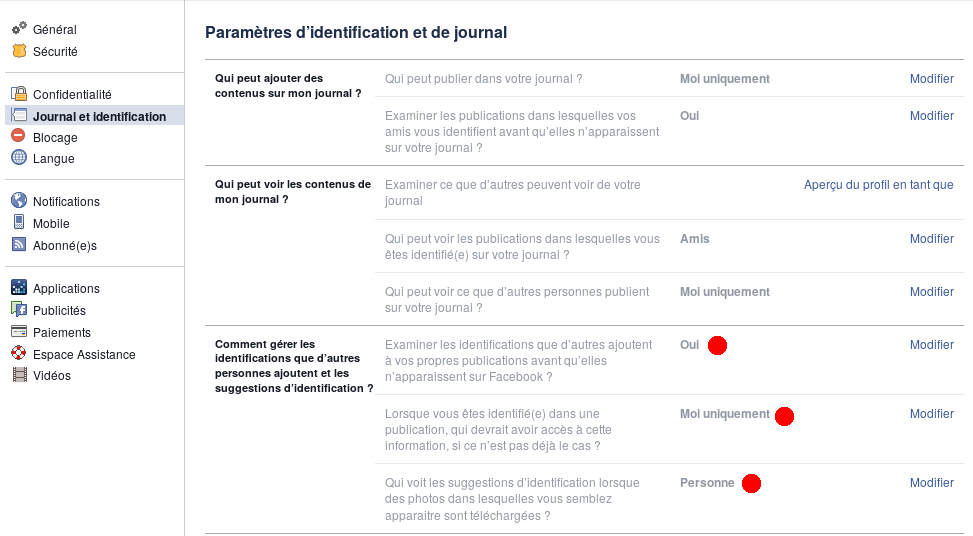
\includegraphics[width=\textwidth,height=\textheight,keepaspectratio]{./privacy-settings.png} 
\end{frame}
}

\begin{frame}
{Déroulement d'une fraude classique}
\begin{itemize}
\item Une connaissance vous ajoute (à nouveau) comme ami
\item Son profile est correct, photos, quelques contenus, etc
\end{itemize}
\end{frame}

{
\hypersetup{
        colorlinks=true,
        linkcolor=white,
        urlcolor=white
}
\setbeamertemplate{headline} {
        \begin{beamercolorbox}[wd=\paperwidth,dp=8pt,ht=12pt,leftskip=.29cm,rightskip=.29cm]{linecolor}
        Donc tout va bien :)
        \hfill
        \insertinstitute
        \end{beamercolorbox}%
}
\begin{frame}
\centering

\includegraphics[width=\textwidth,height=\textheight,keepaspectratio]{./smile-kitten-large.jpg} 
\end{frame}
}

{
\hypersetup{
        colorlinks=true,
        linkcolor=white,
        urlcolor=white
}
\setbeamertemplate{headline} {
        \begin{beamercolorbox}[wd=\paperwidth,dp=8pt,ht=12pt,leftskip=.29cm,rightskip=.29cm]{linecolor}
        \#oupas
        \hfill
        \insertinstitute
        \end{beamercolorbox}%
}
\begin{frame}
\centering

\includegraphics[width=\textwidth,height=\textheight,keepaspectratio]{./When-Kittens-Attack.jpg} 
\end{frame}
}

\begin{frame}
{Hein quoi mais... ?!}
\begin{itemize}
\item Un vieux contact vous rajoute... ?
\note[item]{Facebook n'a pas l'habitude de paumer vos contacts.}
\item Êtes-vous allez voir le profile complet ?
\note[item]{Un bon indice de fraude : profile bancal}
\item ... En fait, connaissez-vous réellement le contact ?
\note[item]{Oui parce que les vrais amis, sur Facebook...}
\end{itemize}
\end{frame}

\begin{frame}
{Mais pourquoi ça se fait ?}
\begin{itemize}
\item "Victime" qui a besoin d'argent
\item "Victime" avec un smartphone bloqué
\item "Victime" avec n'importe quoi
\end{itemize}
\end{frame}

\begin{frame}
{Se prémunir}
\begin{itemize}
\item Réglages de confidentialité
\note[item]{Amis d'amis au plus large}
\item Inspection des profiles
\note[item]{Surtout si ami censé être déjà présent, ou ami d'ami pas trop connu}
\item Si gros doute, demander confirmation par un autre canal
\note[item]{SMS, mail, etc, mais surtout HORS du RS ciblé}
\end{itemize}
\end{frame}

{
\hypersetup{
        colorlinks=true,
        linkcolor=white,
        urlcolor=white
}
\setbeamertemplate{headline} {
        \begin{beamercolorbox}[wd=\paperwidth,dp=8pt,ht=12pt,leftskip=.29cm,rightskip=.29cm]{linecolor}
        Prudence donc !
        \hfill
        \insertinstitute
        \end{beamercolorbox}%
}
\begin{frame}
\centering

\includegraphics[width=\textwidth,height=\textheight,keepaspectratio]{./cautious.jpg} 
\end{frame}
}

\begin{frame}
{Assez parlez de vous}
\centering

\includegraphics[width=\textwidth,height=\textheight,keepaspectratio]{./baby.jpg} 
\end{frame}

{
\setbeamertemplate{footline}{%
	\begin{beamercolorbox}[wd=\paperwidth,dp=8pt,ht=12pt,leftskip=.29cm,rightskip=.3cm]{linecolor}
	\hfill
	\inserttitle
	\end{beamercolorbox}%
}
{
\centering
\begin{frame}
{Questions ?}

\href{https://ethack.org/}{https://ethack.org/} \\
\vspace{0.3cm}
\href{https://www.twitter.com/EthACK_org}{@EthACK\_org} on Twitter \\
\vspace{0.3cm}
\href{https://www.facebook.com/ethack.org}{ethack.org} on Facebook

\vspace{0.5cm}


\includegraphics[width=4cm]{../common/logo_537.png}
\end{frame}
}
}

\end{document}